\begin{homeworkProblem}

\begin{homeworkSubProblem}
    The DFS\&BFS from vertex $a$ are shown in \cref{1.a} and \cref{1.b}.

    \begin{figure}[H]
        \caption{DFS\&BFS for First Graph}\label{1.a}
        \centering
        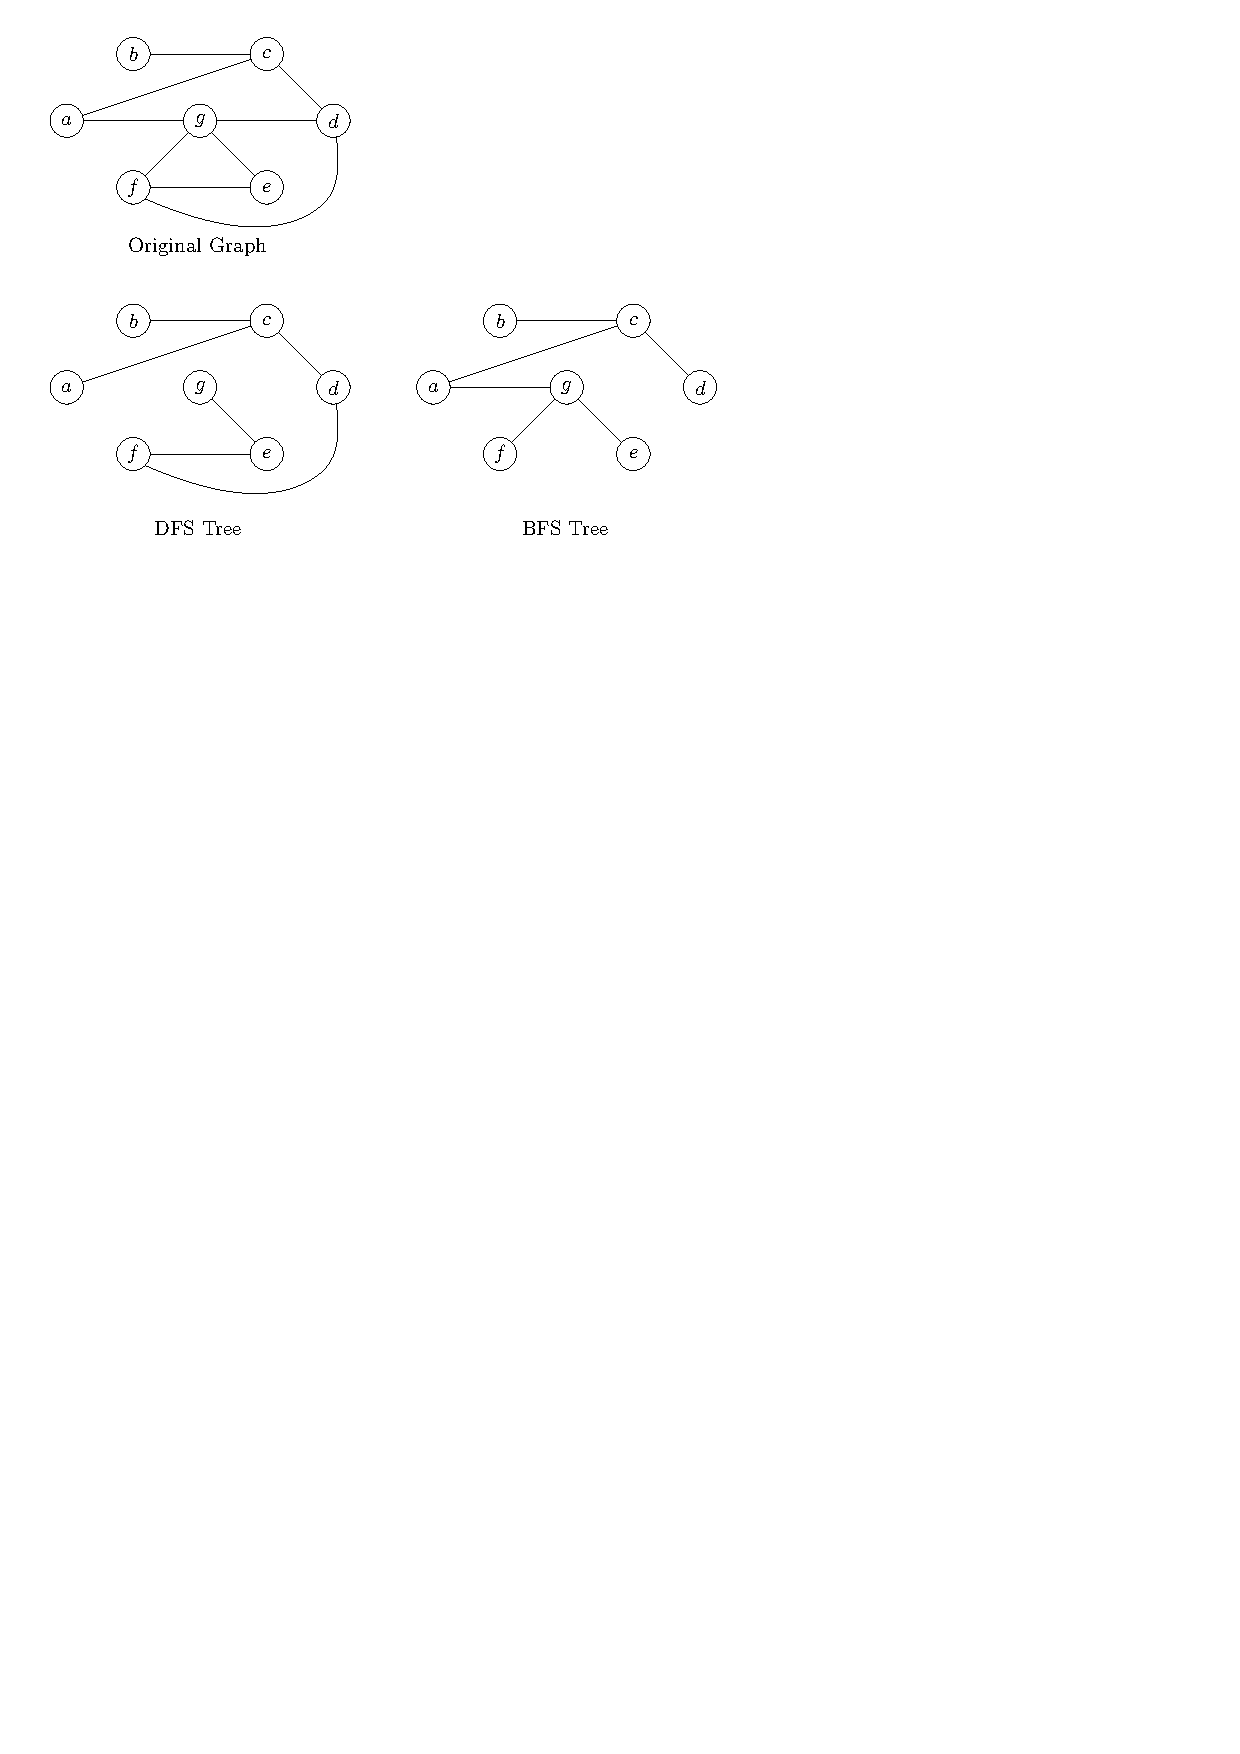
\includegraphics[width=.8\textwidth]{running1a}
    \end{figure}

    \begin{figure}[H]
        \caption{DFS\&BFS for Second Graph}\label{1.b}
        \centering
        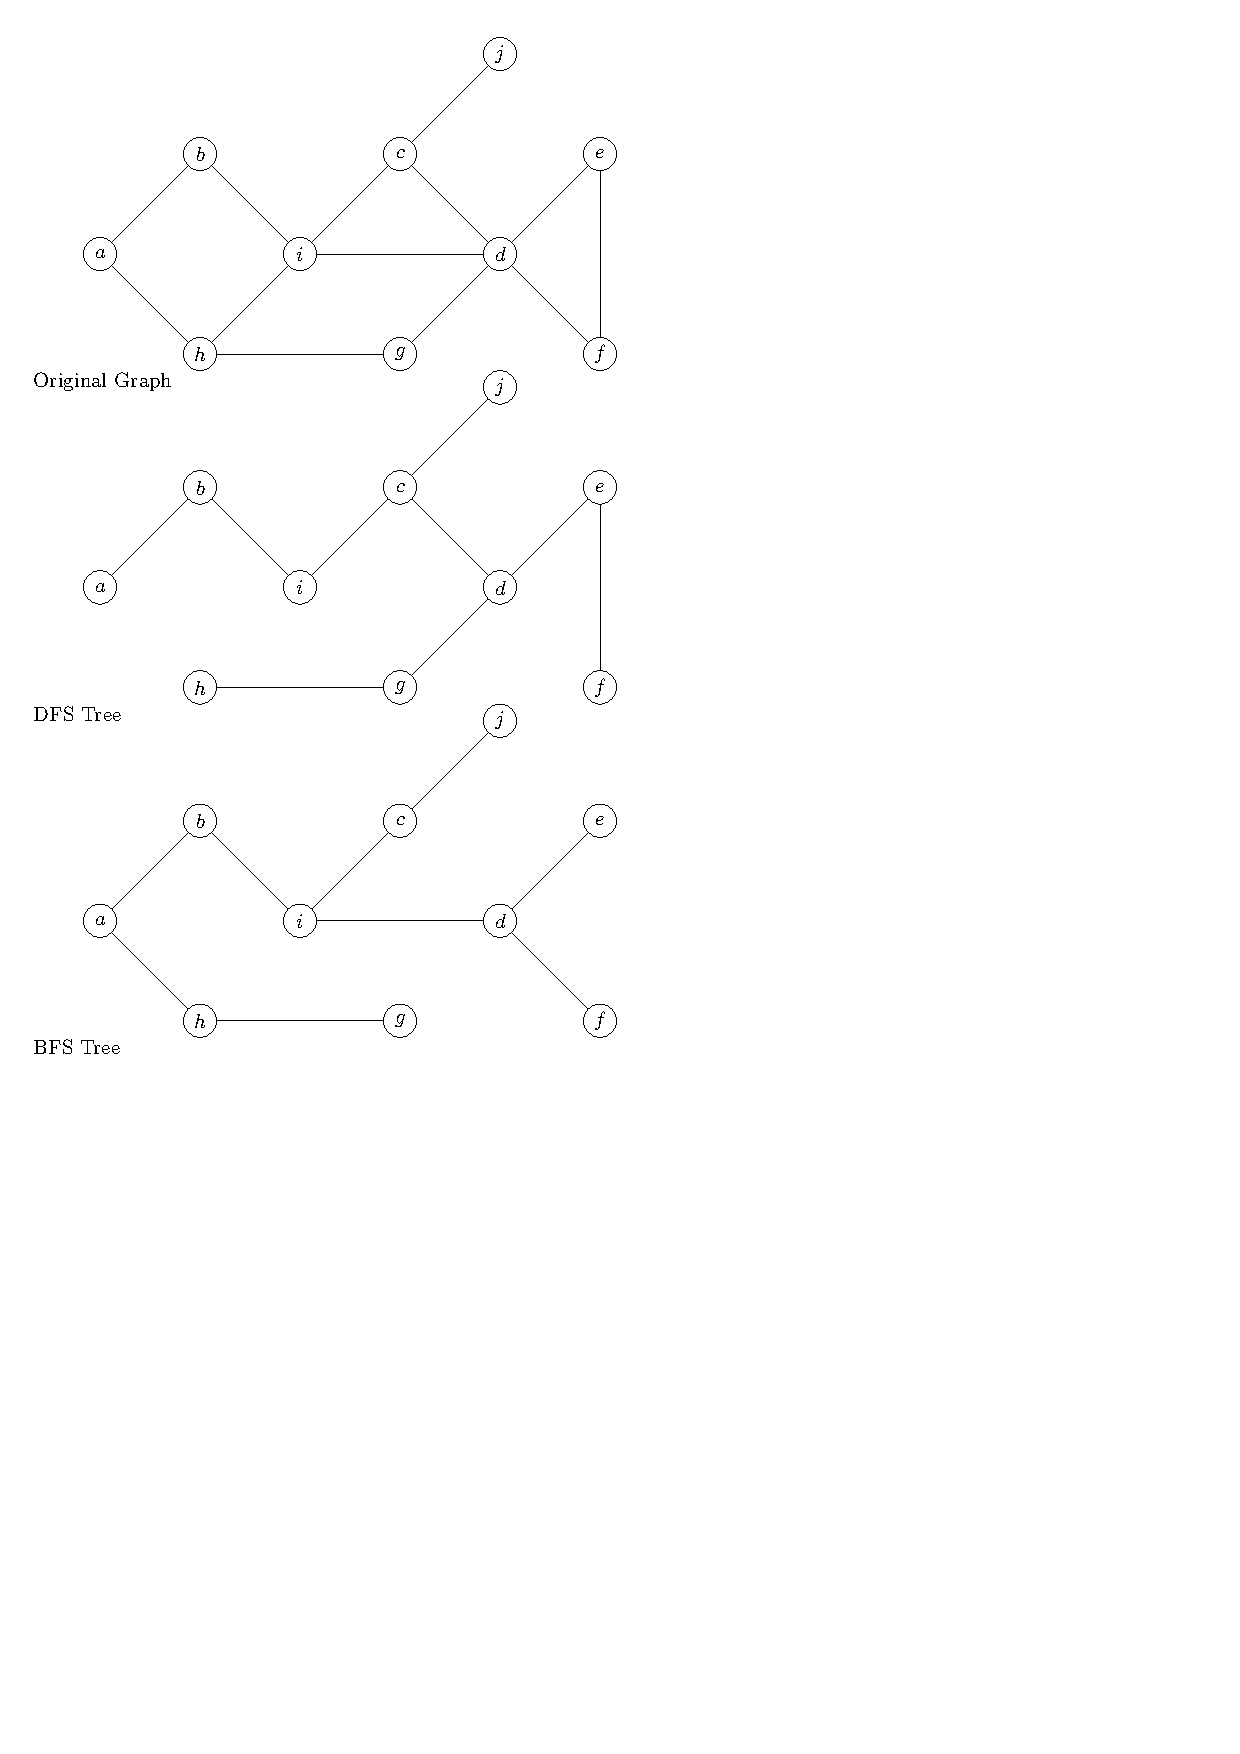
\includegraphics[width=.65\textwidth]{running1b}
    \end{figure}
\end{homeworkSubProblem}

\pagebreak
\begin{homeworkSubProblem}
    The DFS\&BFS from vertex $a$ are shown in \cref{2.a} and \cref{2.b}.

    \begin{figure}[H]
        \caption{Topological Order for First Graph}\label{2.a}
        \centering
        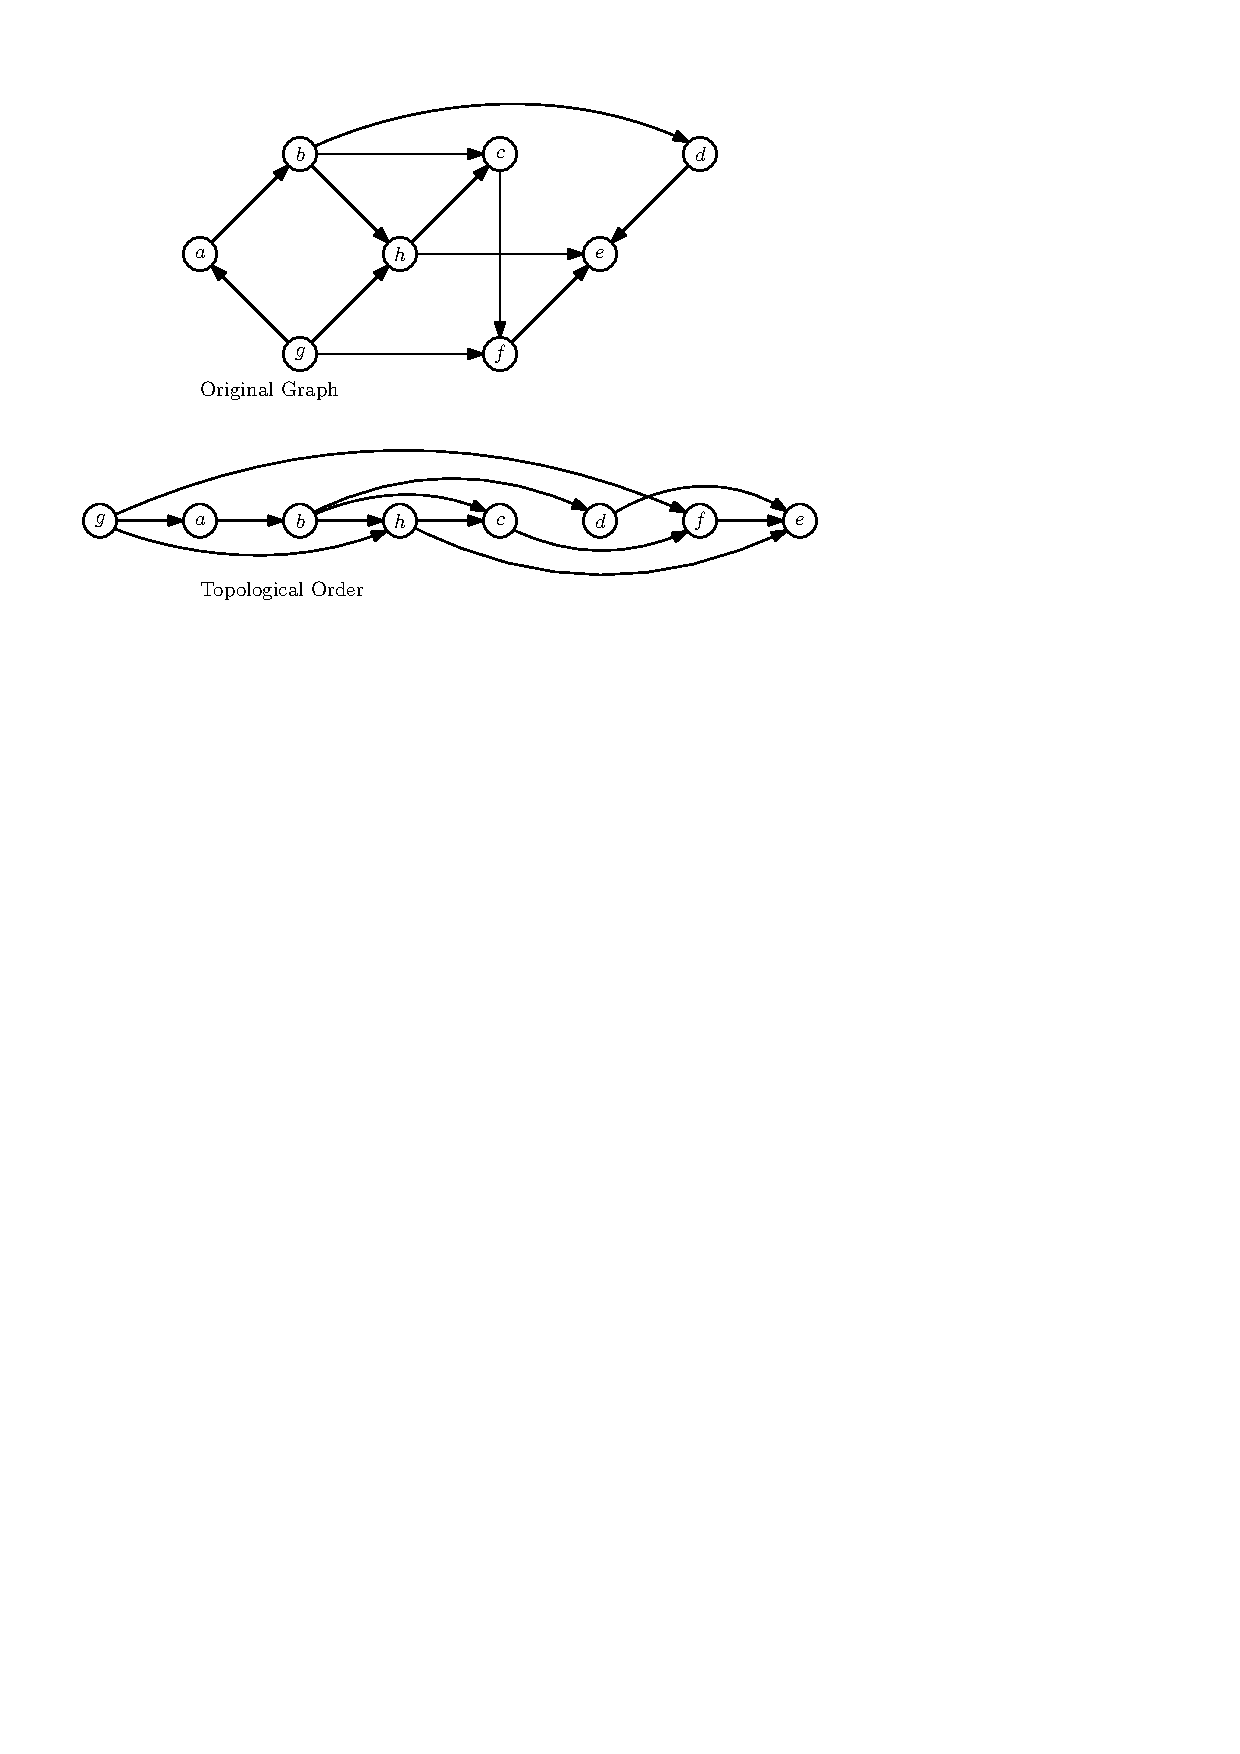
\includegraphics[width=.8\textwidth]{running2a}
    \end{figure}

    \begin{figure}[H]
        \caption{Topological Order for Second Graph}\label{2.b}
        \centering
        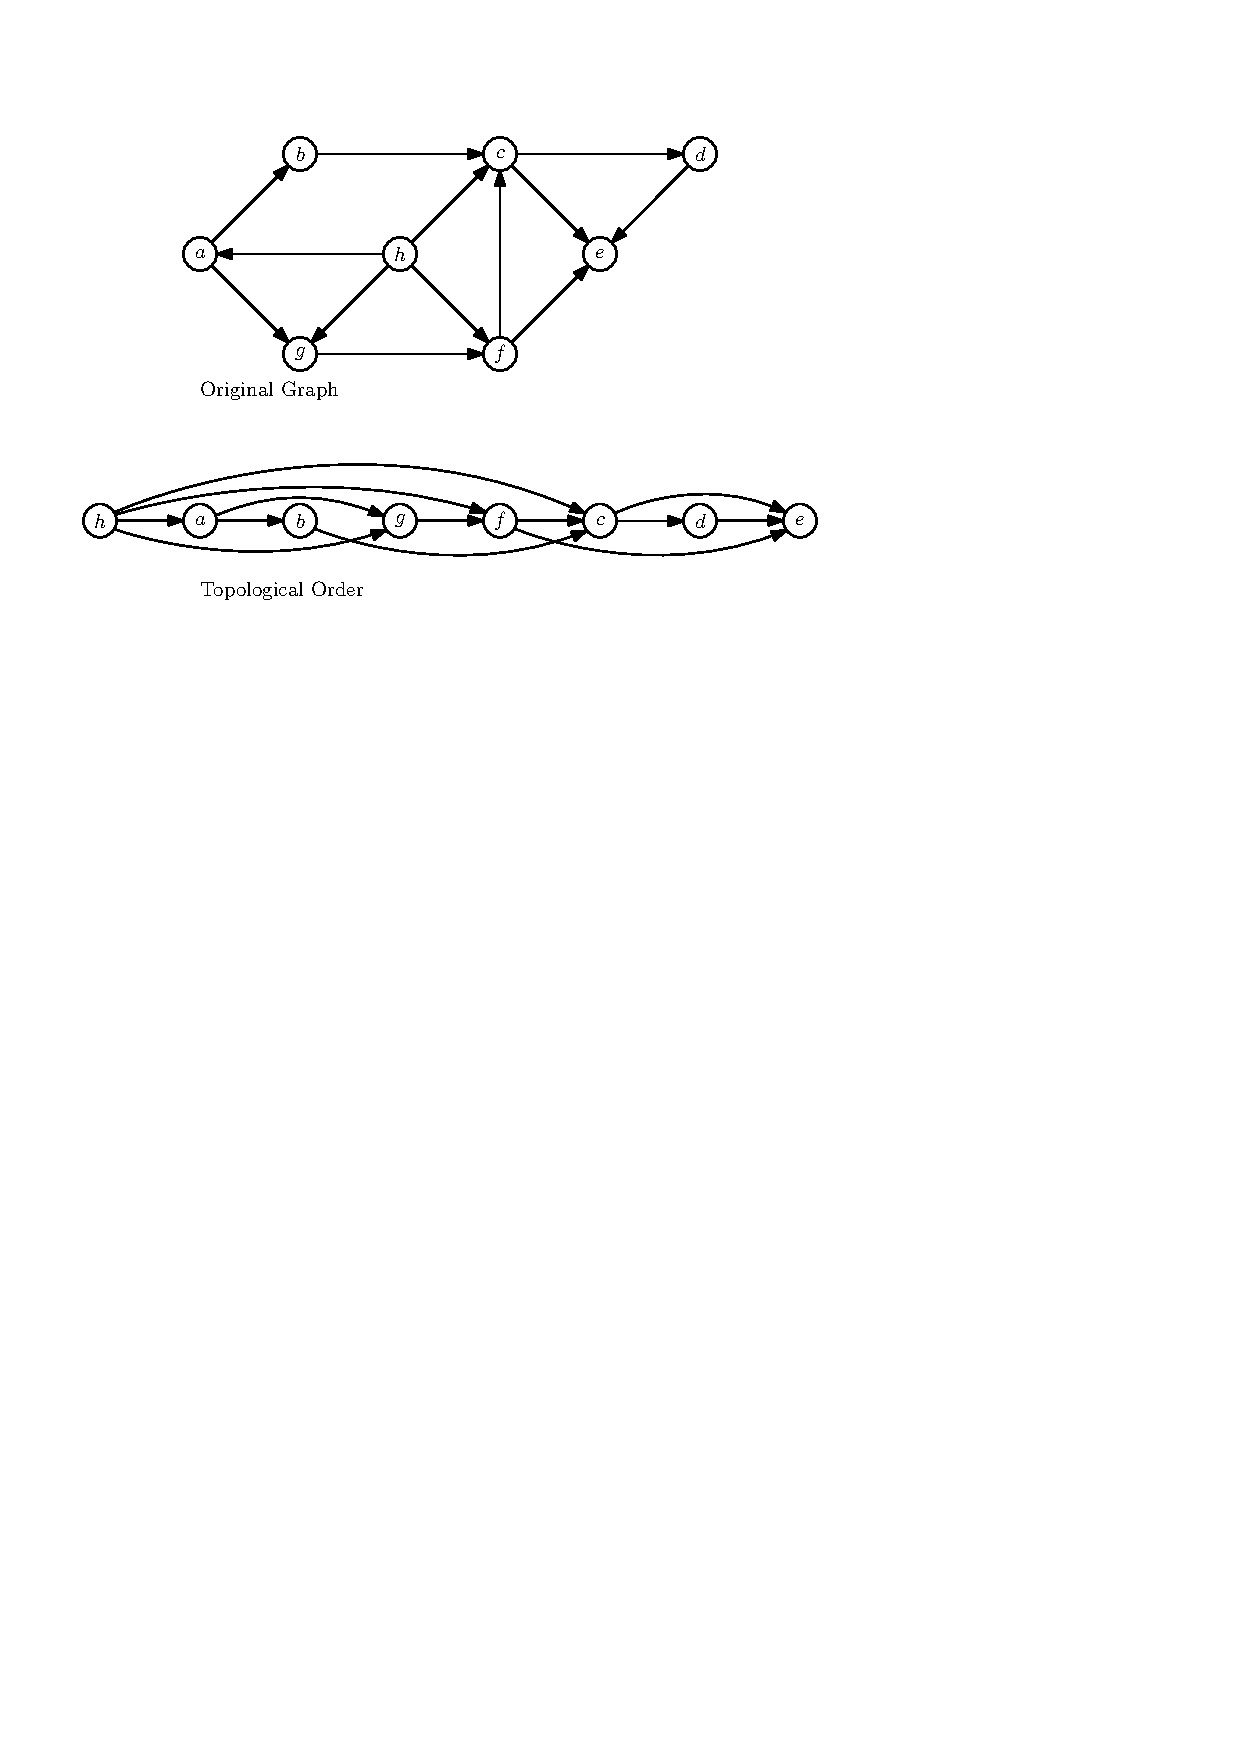
\includegraphics[width=.8\textwidth]{running2b}
    \end{figure}
\end{homeworkSubProblem}

\begin{homeworkSubProblem}
    The MST generation order is shown in \cref{3}, from which we know
    that the weight of the fifth edge added for graph 1 is $3$,
    for graph 2 is $7$.

    \begin{figure}[H]
        \caption{Prim's Algorithm Edge Added Order for First Graph}\label{3}
        \centering
        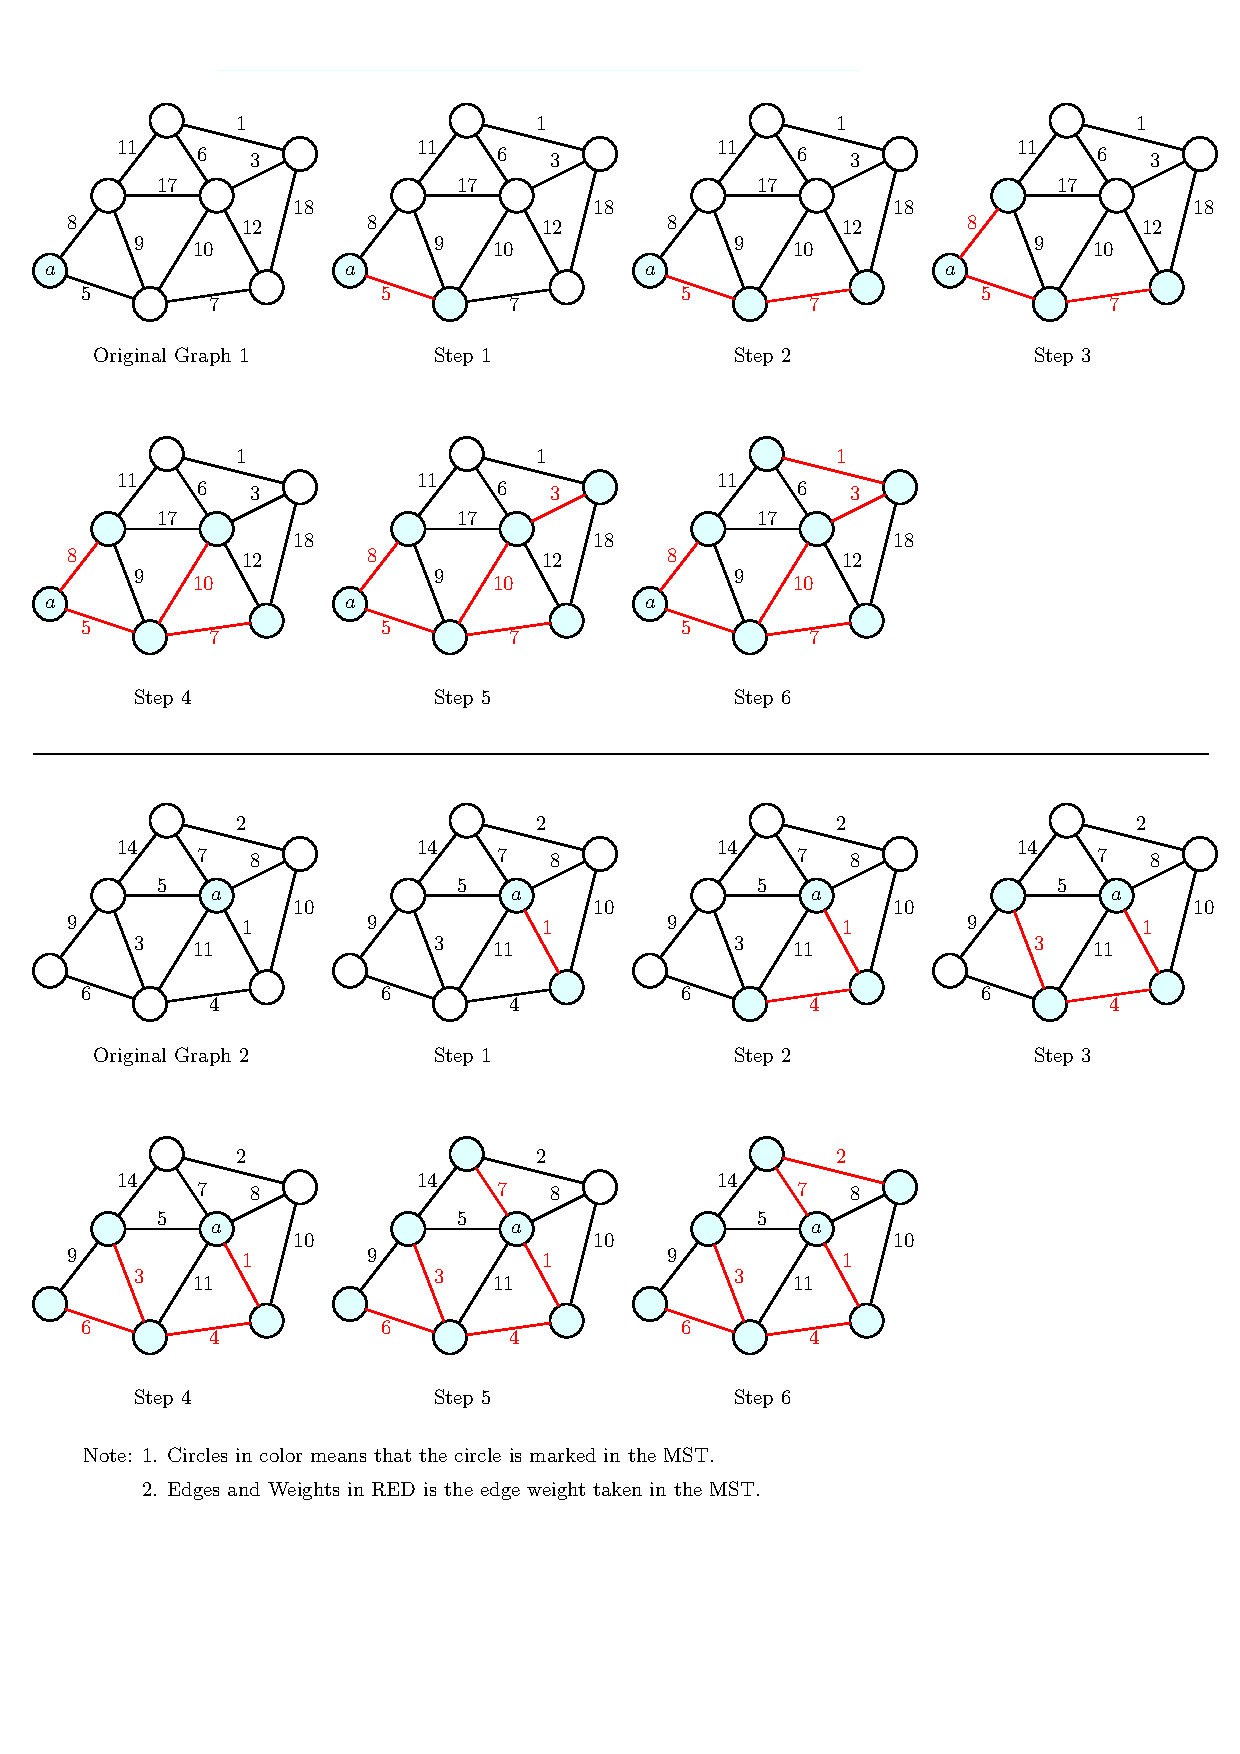
\includegraphics[width=\textwidth]{running3}
    \end{figure}
\end{homeworkSubProblem}

\begin{homeworkSubProblem}
s
    \begin{figure}[H]
        \caption{Prim's Algorithm Edge Added Order for First Graph}\label{4}
        \centering
        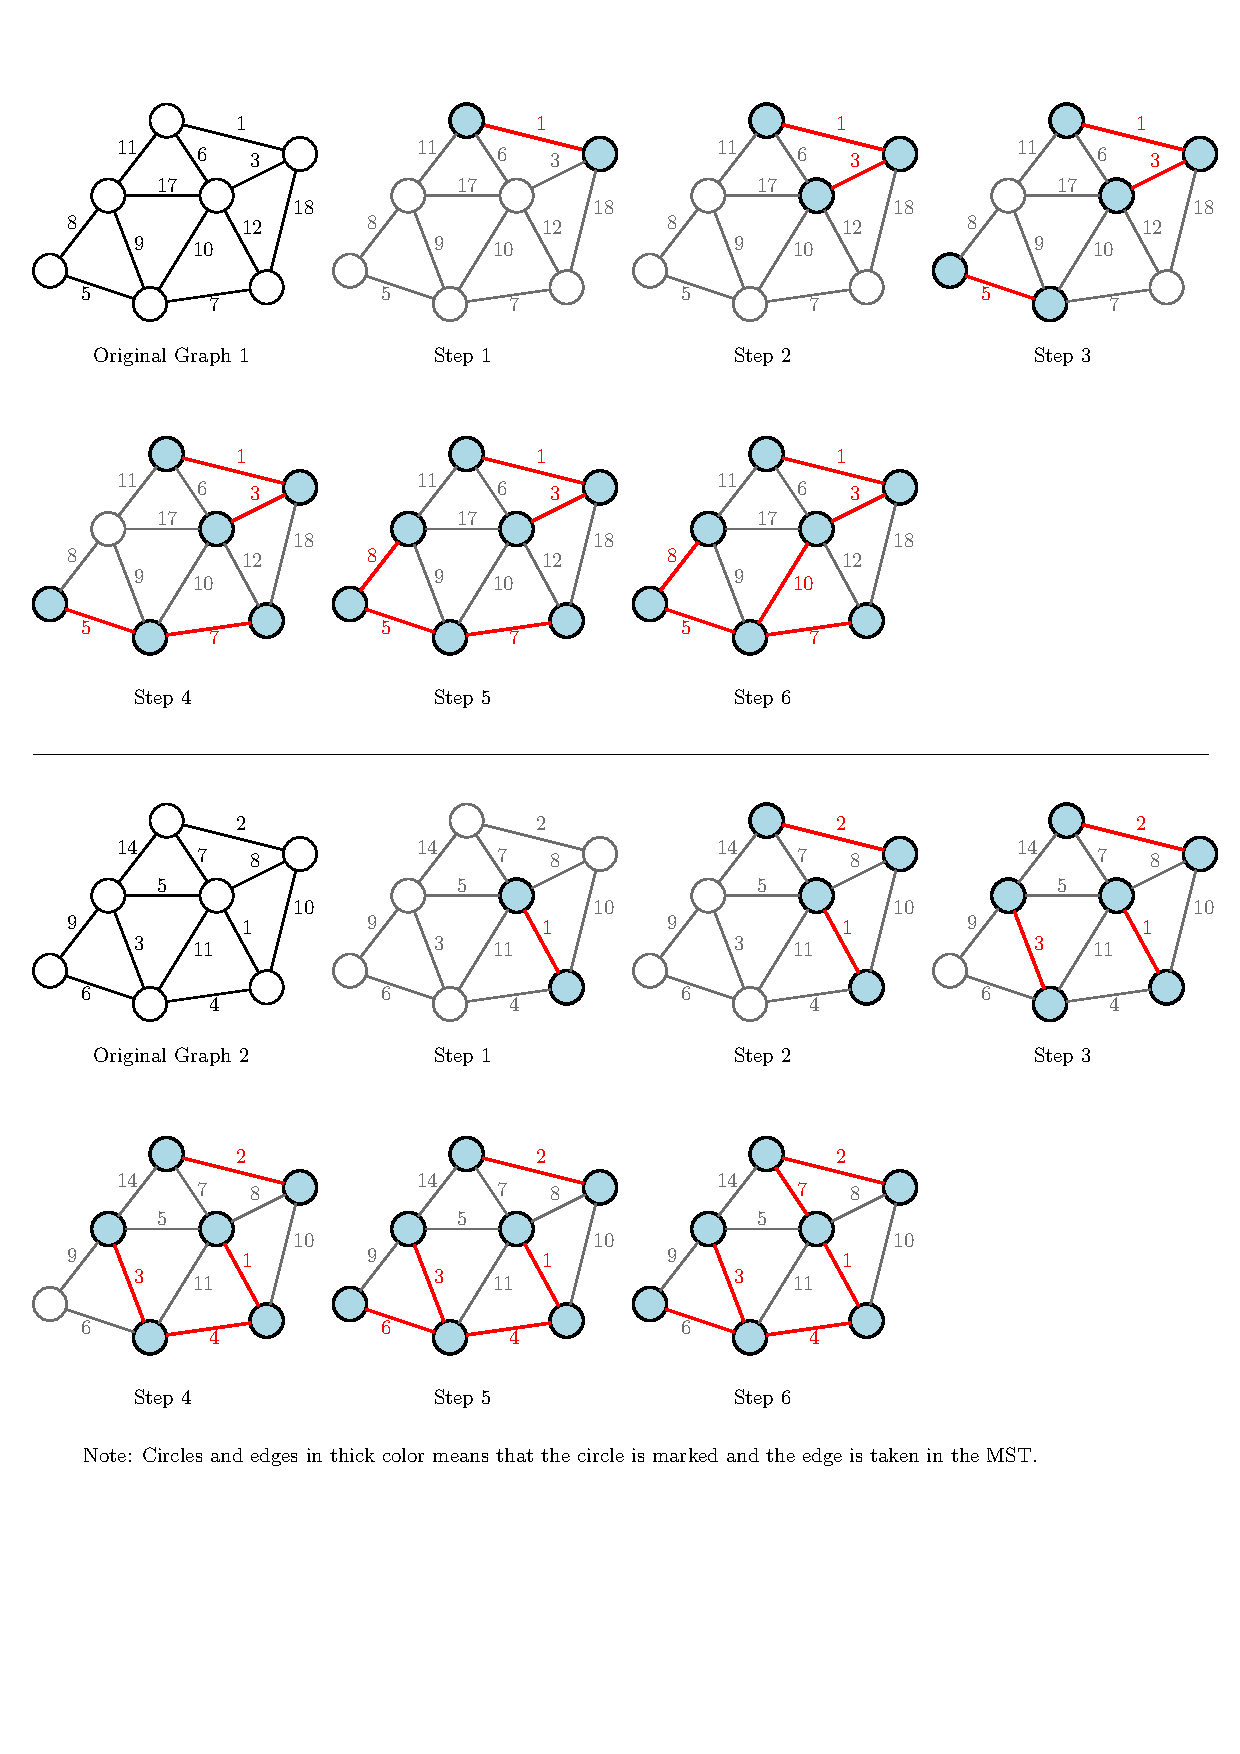
\includegraphics[width=\textwidth]{running4}
    \end{figure}
\end{homeworkSubProblem}
\end{homeworkProblem}
